% INFO-H410 — Automated University Course Scheduling
% Project Report — AAAI 2026 format
\documentclass[letterpaper]{article}
\usepackage{aaai2026}
\usepackage{times}
\usepackage{helvet}
\usepackage{courier}
\usepackage[hyphens]{url}
\usepackage{graphicx}
\urlstyle{rm}
\def\UrlFont{\rm}
\usepackage{natbib}
\usepackage{caption}
\usepackage[hidelinks]{hyperref}
\frenchspacing
\setlength{\pdfpagewidth}{8.5in}
\setlength{\pdfpageheight}{11in}
\pdfinfo{/TemplateVersion (2026.1)}

\usepackage{amsmath,amssymb}
\usepackage{booktabs}
\usepackage{multirow}

\setcounter{secnumdepth}{2}

\title{Automated University Course Scheduling:\\
A Comparative Study of CSP, Local Search, and Q-Learning}

\author{
    Nassim Machichi,
    Urielle Nkwinga,
    Burak Sogutlu,
    Gr\'{e}goire Van den Eynde
}
\affiliations{
    Groupe 9 --- MA1 Ing\'{e}nieur Civil, Universit\'{e} Libre de Bruxelles\\
    INFO-H410, Techniques of Artificial Intelligence, 2025/2026\\
    \url{https://github.com/BurakSogutlu/Project-TAI-25-26-course_scheduler}
}

\begin{document}
\maketitle

\begin{abstract}
We compare three AI techniques for university course scheduling: a Constraint Satisfaction Problem (CSP) solver with backtracking and heuristics, Simulated Annealing (SA), and a tabular Q-Learning agent. Seven benchmark instances from 5 to 150 courses are evaluated on hard-constraint violations, soft-preference score, and runtime. CSP guarantees zero constraint violations with high solution quality up to 125 courses, but becomes intractable beyond that point. SA handles all instance sizes in under 5 seconds, at the cost of some hard violations on dense problems. Q-Learning is fundamentally limited by the curse of dimensionality and is not competitive in this setting. All code and data are available at the repository linked above.
\end{abstract}

\section{Introduction and Problem Formulation}

University timetabling is a classic combinatorial optimisation problem. Given a set of courses, professors, rooms, and time slots, the goal is to produce a schedule satisfying a set of hard constraints while maximising soft preferences. The problem is NP-hard in general \cite{russell2020}, which makes it a natural testbed for comparing exact, heuristic, and learning-based approaches.

\subsection{Formal Definition}

Let $\mathcal{C}$, $\mathcal{P}$, $\mathcal{R}$, $\mathcal{T}$ denote the sets of courses, professors, rooms, and time slots. The week is divided into 20 slots (5 days $\times$ 4 blocks). A solution is a total assignment $\sigma: \mathcal{C} \rightarrow \mathcal{R} \times \mathcal{T}$ satisfying the following hard constraints:
\begin{itemize}
    \item (H1) No professor teaches two simultaneous courses.
    \item (H2) No room hosts two simultaneous courses.
    \item (H3) Each room has sufficient capacity for its assigned course.
    \item (H4) Each course is placed in a slot where its professor is available.
    \item (H5) No professor exceeds a daily course limit.
\end{itemize}

The soft objective rewards scheduling in professors' preferred slots and balancing the weekly load. The combined objective used throughout is $\mathcal{F}(\sigma) = -10 \cdot |\text{violations}| + \text{soft\_score}(\sigma)$, where the soft score is normalised to $[0,1]$. The large penalty coefficient ensures that any hard violation dominates any soft gain, so all three approaches effectively minimise violations first and then optimise quality.

\subsection{Search Space and Complexity}

The theoretical search space is the product of all possible (room, slot) assignments for each course: $|\mathcal{R} \times \mathcal{T}|^{|\mathcal{C}|}$. Even after filtering with unary constraints H3 and H4, which typically reduce each domain to around 60\% of all (room, slot) pairs, this remains enormous. For instance\_30 with 30 courses, 8 rooms and 20 slots, a rough lower bound on the search space is $(0.6 \times 160)^{30} \approx 10^{70}$ distinct assignments. This figure illustrates why exhaustive enumeration is impossible and why heuristics, pruning, or approximation are all necessary.

The constraint graph provides another useful perspective. Constraints H1 and H2 define binary constraints between pairs of courses. Two courses sharing a professor are always in conflict under H1. Two courses sharing a room at the same slot are in conflict under H2. On instance\_125, with 25 professors each teaching an average of 5 courses, H1 alone creates approximately $25 \times \binom{5}{2} = 250$ conflict pairs, before even considering room conflicts. This dense constraint graph is the direct cause of the exponential growth in CSP backtracking time visible in Figure~\ref{fig:time}.

\subsection{Benchmark Instances}

All three approaches are evaluated on the same seven pre-generated instances (Table~\ref{tab:instances}), serialised to JSON with a fixed random seed. Using fixed instances guarantees that differences in results reflect algorithmic behaviour rather than instance difficulty.

\begin{table}[h]
\centering
\caption{Benchmark instances used in all experiments.}
\label{tab:instances}
\small
\begin{tabular}{@{}lrrrl@{}}
\toprule
Instance & Courses & Profs & Rooms & Notes \\
\midrule
instance\_05  &   5 &  3 &  3 & Toy/sanity check \\
instance\_15  &  15 &  6 &  5 & Small \\
instance\_30  &  30 & 10 &  8 & Medium \\
instance\_60  &  60 & 15 &  8 & Medium-large \\
instance\_100 & 100 & 20 &  8 & Large \\
instance\_125 & 125 & 25 &  8 & Near CSP limit \\
instance\_150 & 150 & 30 &  8 & CSP failure zone \\
\bottomrule
\end{tabular}
\end{table}

\section{Approach A: CSP with Backtracking}

The scheduling problem maps naturally onto a CSP \cite{russell2020}: each course is a variable, and its domain is the set of (room, slot) pairs satisfying the unary constraints H3 and H4, filtered once at startup. The binary constraints H1 and H2 link pairs of courses sharing a professor or competing for the same room.

\subsection{Heuristics}

The solver uses recursive backtracking augmented with three heuristics. MRV (Minimum Remaining Values) selects the most constrained variable next, reducing the risk of late-stage dead ends. The Degree heuristic breaks MRV ties by preferring the course with the most constraints on other unassigned courses. LCV (Least Constraining Value) is repurposed here as a soft-constraint optimiser: candidate (room, slot) pairs are sorted by descending soft score rather than by how little they eliminate from neighbouring domains. As a result, the very first complete schedule found by the search is already close to optimal, without any post-processing step.

\subsection{Constraint Propagation}

For constraint propagation, we use Forward Checking (FC) rather than full AC-3 arc-consistency. FC eliminates values from the domains of unassigned neighbours after each assignment, detecting dead ends early at a cost of $O(d)$ per step. AC-3 provides stronger propagation at a cost of $O(cd^3)$ by iterating over all arcs until no further pruning is possible. In practice, FC with MRV and Degree achieved zero backtracks on every instance up to 125 courses (Figure~\ref{fig:viol}), showing that the variable-ordering heuristics are sufficient to avoid dead ends on our benchmark, making the additional overhead of AC-3 unnecessary.

\subsection{Anytime Variant}

An Anytime variant was also implemented: it records the best solution found so far and continues searching beyond the first complete schedule until a time budget expires. Because the LCV soft-score trick makes the first solution already near-optimal, the Anytime variant never finds a meaningfully better second solution within its budget (Figure~\ref{fig:soft}). A further subtlety: if the timeout expires before the first solution is found (for instance, a 30\,s budget on instance\_100 which requires 41\,s, as seen in Figure~\ref{fig:time}), the Anytime variant returns nothing at all, performing strictly worse than the standard solver. This highlights the importance of calibrating the timeout to the expected difficulty of the instance.

\section{Approach B: Local Search (Simulated Annealing)}

Unlike CSP, local search starts from a complete but potentially invalid schedule: each course is randomly assigned to any (slot, room) pair, ignoring all constraints. The search then iteratively improves $\mathcal{F}$ by exploring neighbouring schedules.

\subsection{Neighbourhood Operators}

Two neighbourhood operators are applied with equal probability at each step. The Move operator reassigns one randomly chosen course to a new random (slot, room) pair. The Swap operator exchanges the full assignments of two randomly chosen courses. Both produce a new complete schedule in constant time and together form a connected neighbourhood, meaning any valid schedule is reachable in principle.

\subsection{Hill Climbing and Simulated Annealing}

We first implemented a Hill Climbing baseline that only accepts improvements ($\Delta\mathcal{F} > 0$). While fast to converge on small instances, it consistently gets trapped in local optima on larger ones, returning schedules with many hard violations. Simulated Annealing addresses this by also accepting worsening moves with probability $e^{\Delta\mathcal{F}/T}$, where $T$ is a temperature that decreases over time. Starting at $T_0 = 10.0$ with a cooling rate of $0.995$, the temperature after 4\,000 iterations is approximately $1.7 \times 10^{-9}$, effectively freezing the search at a local optimum. The best schedule seen across all iterations is returned as the final solution. SA consistently outperforms Hill Climbing in both solution quality (Figure~\ref{fig:soft}) and constraint satisfaction (Figure~\ref{fig:viol}), confirming the practical benefit of probabilistic acceptance.

\section{Approach C: Q-Learning}

Q-Learning formulates the scheduling problem as a sequential Markov Decision Process. Each episode builds one complete schedule from scratch: courses are placed one at a time in shuffled order, and the agent chooses a (slot, room) pair for each course. The reward after each placement is the current value of $\mathcal{F}$, immediately reflecting whether the assignment introduced new violations or satisfied preferences.

\subsection{State Representation}

Maintaining a full Q-table over all possible partial schedules is intractable, since the state space grows combinatorially with the number of courses. To make the approach feasible, each (course, slot, room, partial schedule) configuration is represented by a compact 5-dimensional feature vector: whether the slot is in the professor's preferred slots, whether the professor already teaches at that slot, whether the room is already occupied, the number of courses already scheduled on that day, and whether the room has sufficient capacity. This reduces the effective Q-table size from exponential to a manageable constant-width representation. However, this compression comes at a cost: many distinct scheduling states map to the same feature vector, causing the agent to confuse different situations and learn suboptimal policies.

\subsection{Training}

The agent uses $\varepsilon$-greedy exploration: with probability $\varepsilon$ it picks a random action, otherwise it exploits the action with the highest Q-value for the current feature vector. $\varepsilon$ decays linearly from 1.0 to 0.05 over all episodes. Q-values are updated after each placement via the Bellman equation:
\[
Q(s,a) \leftarrow Q(s,a) + \alpha\big[r + \gamma \max_{a'}Q(s',a') - Q(s,a)\big]
\]
with $\alpha = 0.1$ and $\gamma = 0.9$.

Even with this compression, the number of training episodes must be drastically reduced on large instances, from 1\,000 episodes for $n = 5$ down to just 2 for $n > 100$, to prevent unbounded runtimes. At that scale, the agent has no opportunity to learn a useful policy, and its decisions are essentially random, which directly explains the explosion in violations observed in Figure~\ref{fig:viol} and the collapse in soft score visible in Figure~\ref{fig:soft}. This is the core limitation of tabular Q-Learning on combinatorial scheduling: the feature representation loses global context, and the episode budget prevents meaningful exploration.

\section{Experimental Evaluation}
\label{sec:eval}

The CSP Anytime timeout was set to 30\,s. SA used 4\,000 iterations for small instances, scaling down to 500 for $n > 100$. Q-Learning used 1\,000 episodes for $n \leq 5$, 50 for $n \leq 25$, and 2 for $n > 100$.

\begin{table}[h]
\centering
\caption{Selected results (Viol. = hard violations, SS = soft score).}
\label{tab:results}
\small
\begin{tabular}{@{}llrrr@{}}
\toprule
Instance & Algorithm & Time (s) & Viol. & SS \\
\midrule
\multirow{3}{*}{05 (5c)}   & CSP &  0.01 &  0 & 0.867 \\
                            & SA  &  0.45 &  0 & 0.867 \\
                            & QL  &  5.13 &  0 & 0.733 \\
\midrule
\multirow{3}{*}{30 (30c)}  & CSP &  3.05 &  0 & 0.633 \\
                            & SA  &  1.59 &  0 & 0.522 \\
                            & QL  & 10.75 &  3 & 0.244 \\
\midrule
\multirow{3}{*}{100 (100c)}& CSP & 41.44 &  0 & 0.313 \\
                            & SA  &  4.34 &  8 & 0.090 \\
                            & QL  & 33.25 & 50 & 0.107 \\
\midrule
\multirow{2}{*}{125 (125c)}& CSP & 61.12 &  0 & 0.189 \\
                            & SA  &  3.71 & 56 & 0.075 \\
\midrule
\multirow{2}{*}{150 (150c)}& SA  &  2.62 & 72 & 0.056 \\
                            & QL  &  4.34 &109 & 0.053 \\
\bottomrule
\end{tabular}
\end{table}

Table~\ref{tab:results} summarises the key results. The CSP produces the best outcome on every instance it solves: zero violations and the highest soft score in all cases. SA matches CSP's violation count on small instances but its soft score is consistently lower, a consequence of starting from a random initially invalid schedule rather than building a preference-aware solution from scratch. Q-Learning is only competitive on the 5-course toy instance; beyond that, the combination of insufficient training and a lossy feature representation leads to rapidly degrading results.

\subsection{Runtime}

\begin{figure}[h]
\centering
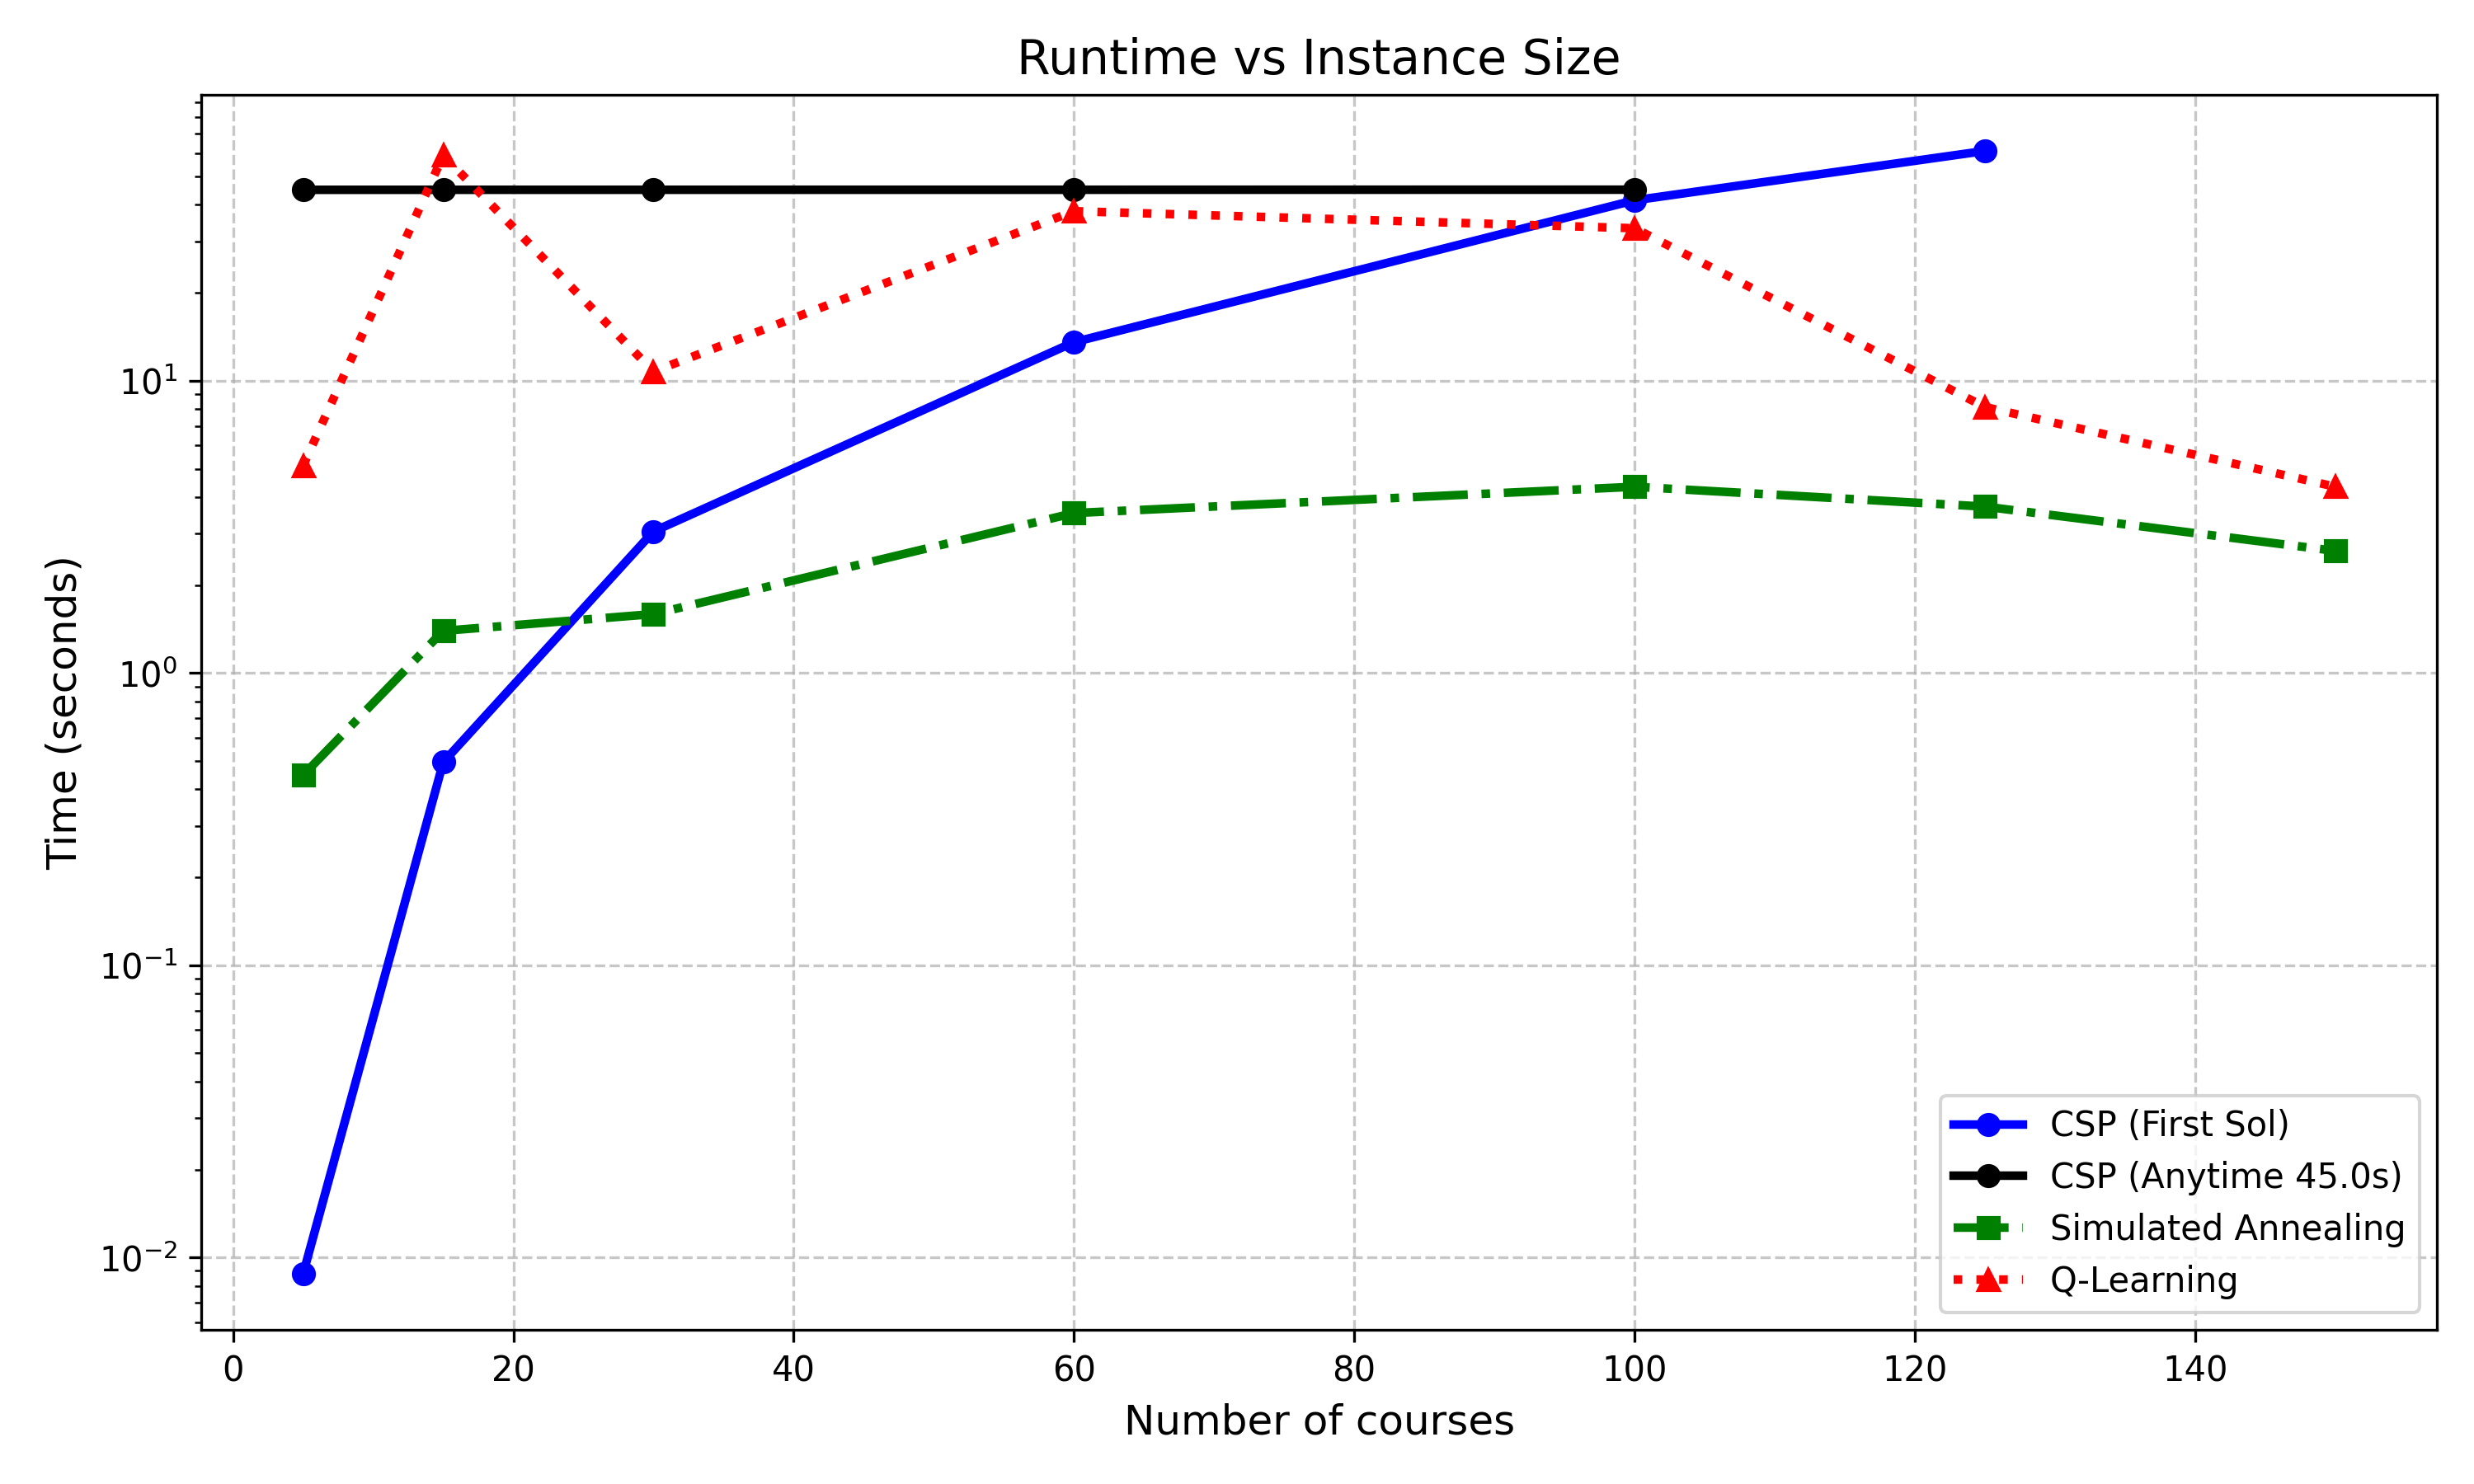
\includegraphics[width=0.95\columnwidth]{Images/time.png}
\caption{Runtime (log scale) vs.\ number of courses.}
\label{fig:time}
\end{figure}

Figure~\ref{fig:time} shows how runtime scales with instance size. CSP grows from 3\,s at $n=30$ to 61\,s at $n=125$, and was confirmed to hang at $n=150$. SA stays below 5\,s regardless of size. Q-Learning's runtime appears to decrease on large instances, but this is entirely due to episode truncation: with only 2 training passes, the agent processes the instance in a fraction of the time it would need to learn anything useful.

\subsection{Solution Quality}

\begin{figure}[h]
\centering
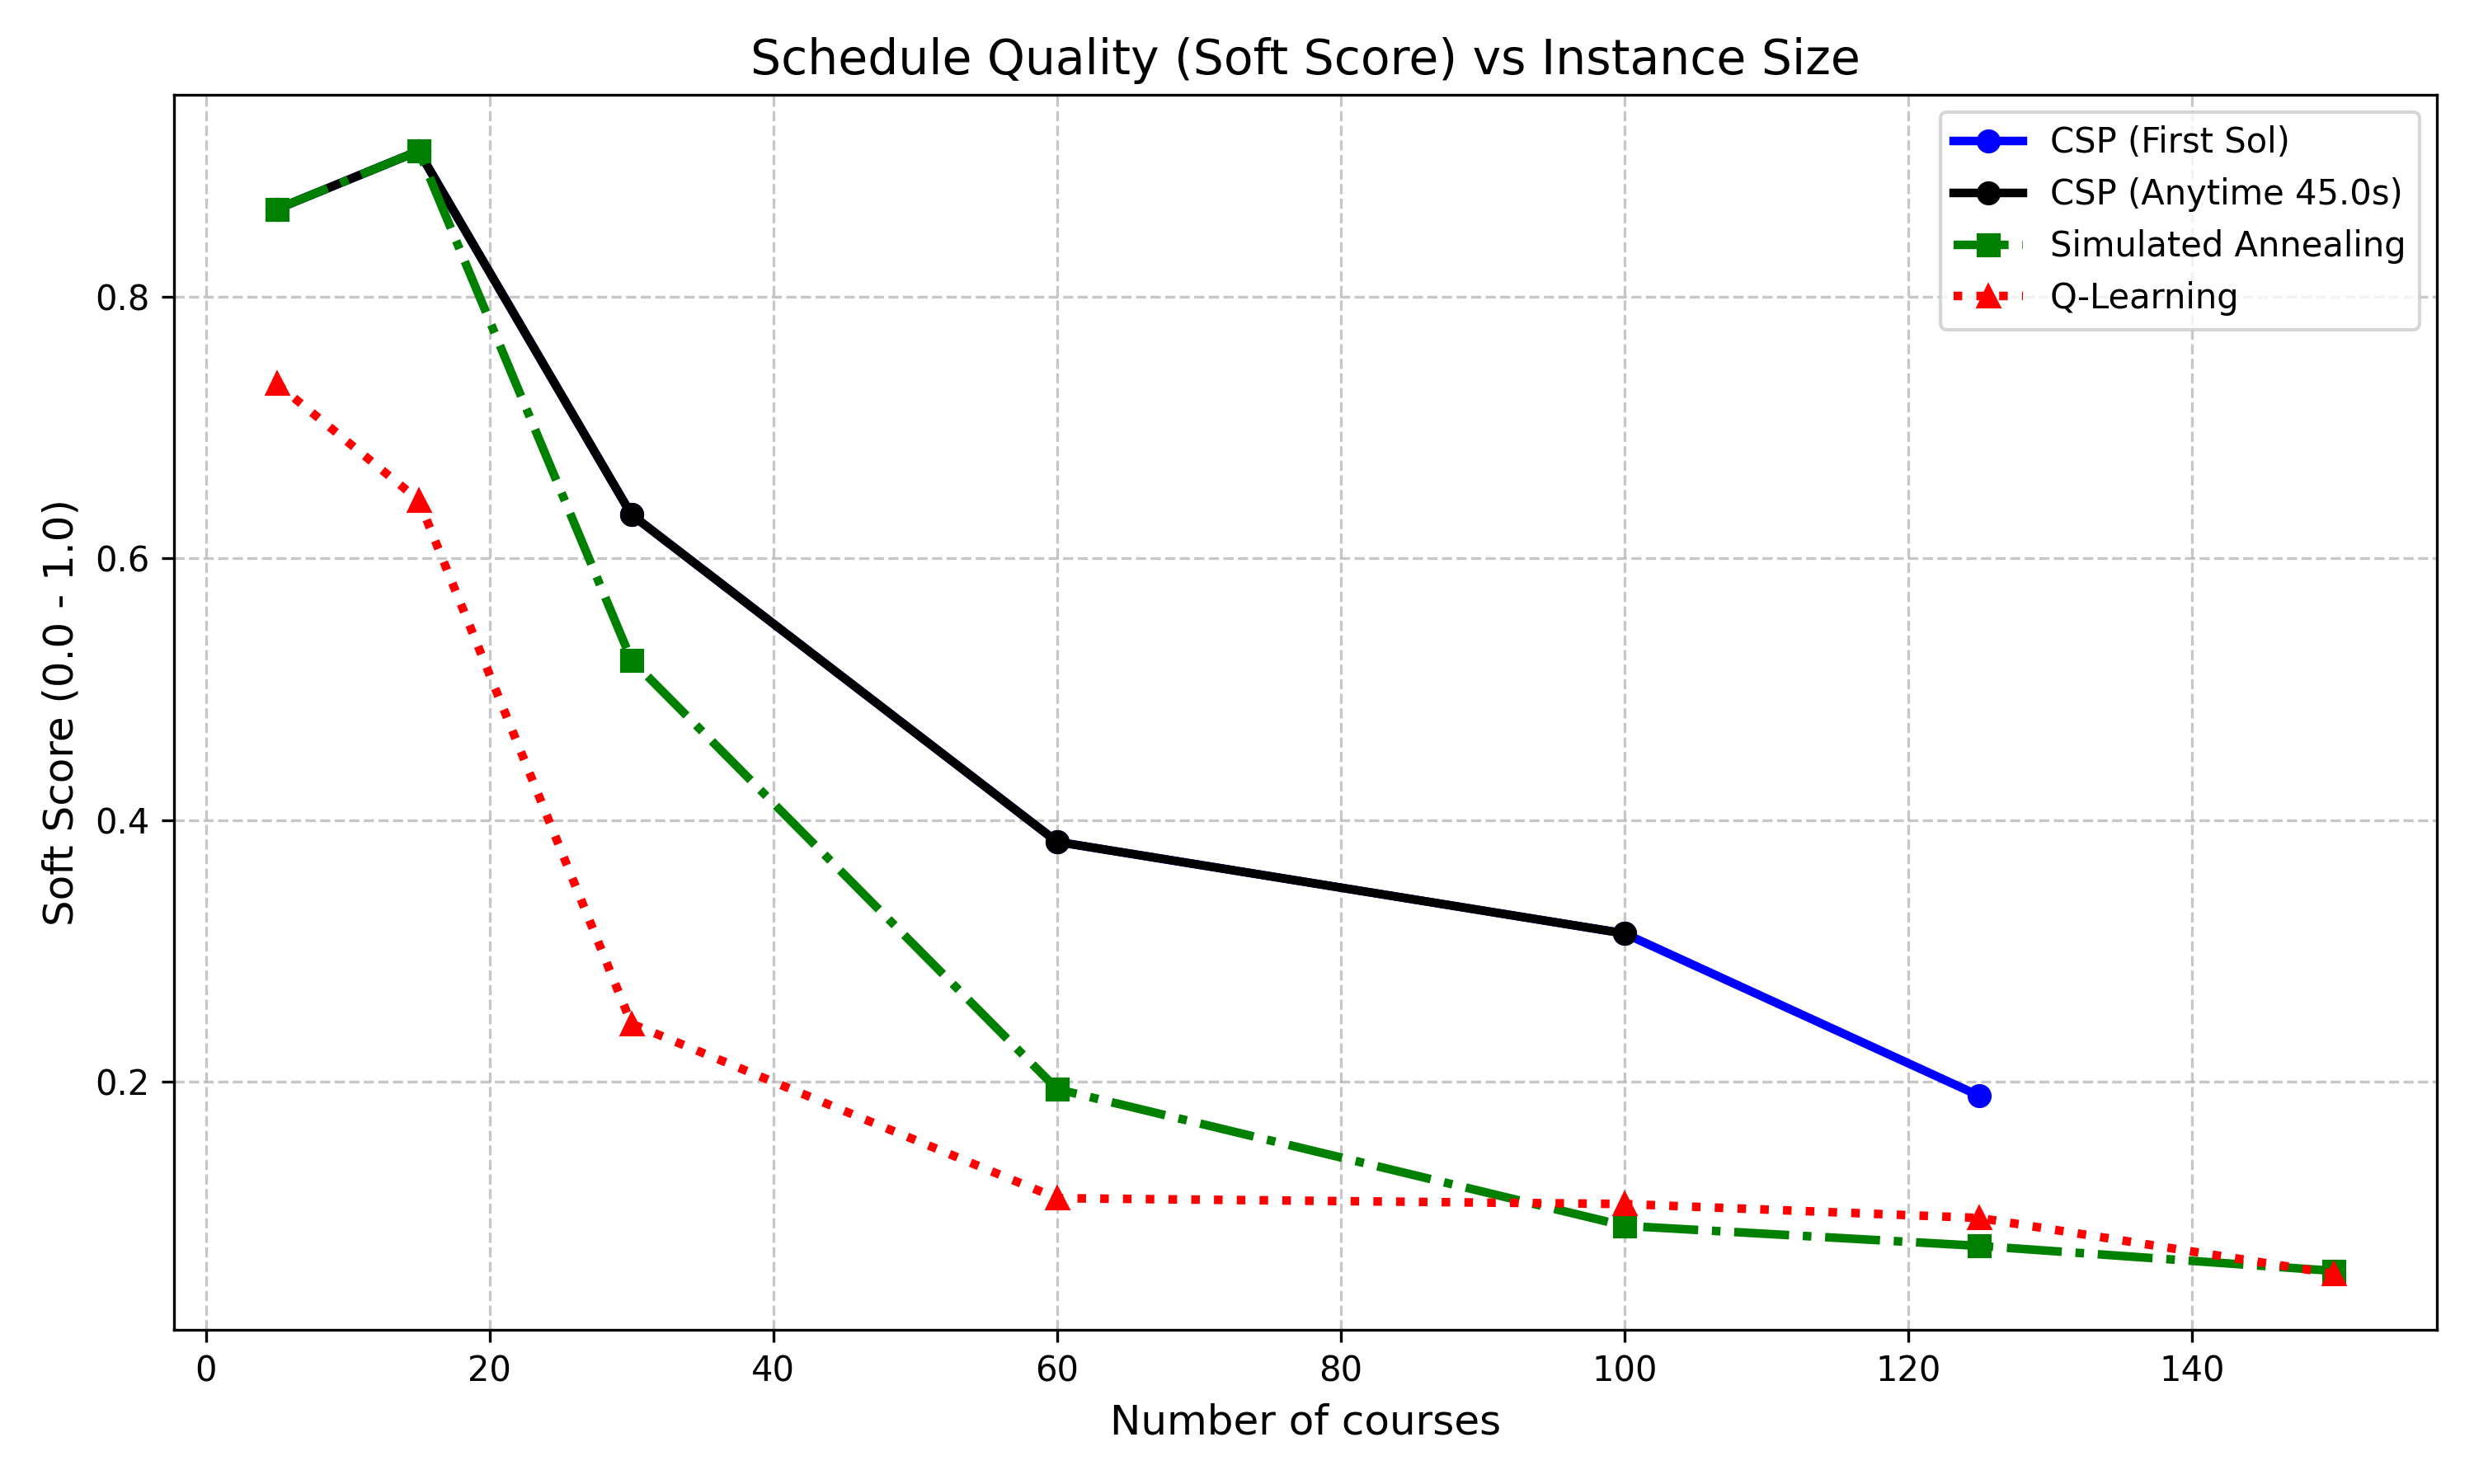
\includegraphics[width=0.95\columnwidth]{Images/soft_score.png}
\caption{Soft score vs.\ number of courses.}
\label{fig:soft}
\end{figure}

Figure~\ref{fig:soft} shows solution quality across all instances. CSP First Sol and CSP Anytime always report identical scores: the LCV soft-score trick makes the first backtracking solution already near-optimal, and the Anytime variant never finds a better second solution within 30\,s. SA's quality drops noticeably from $n=60$ onward as the search space becomes too large for the fixed iteration budget to explore thoroughly. It is also worth noting that the soft score values reflect the structure of each instance as much as the algorithm quality: on instance\_05, both CSP and SA achieve 0.867, indicating that the instance itself cannot allow all preferences to be satisfied simultaneously. This ceiling effect worsens as density grows, with CSP scoring only 0.189 on instance\_125, not because the algorithm degrades, but because with 125 courses competing for 20 slots and 8 rooms, very few preferences can be accommodated.

\subsection{Hard Constraint Violations}

\begin{figure}[h]
\centering
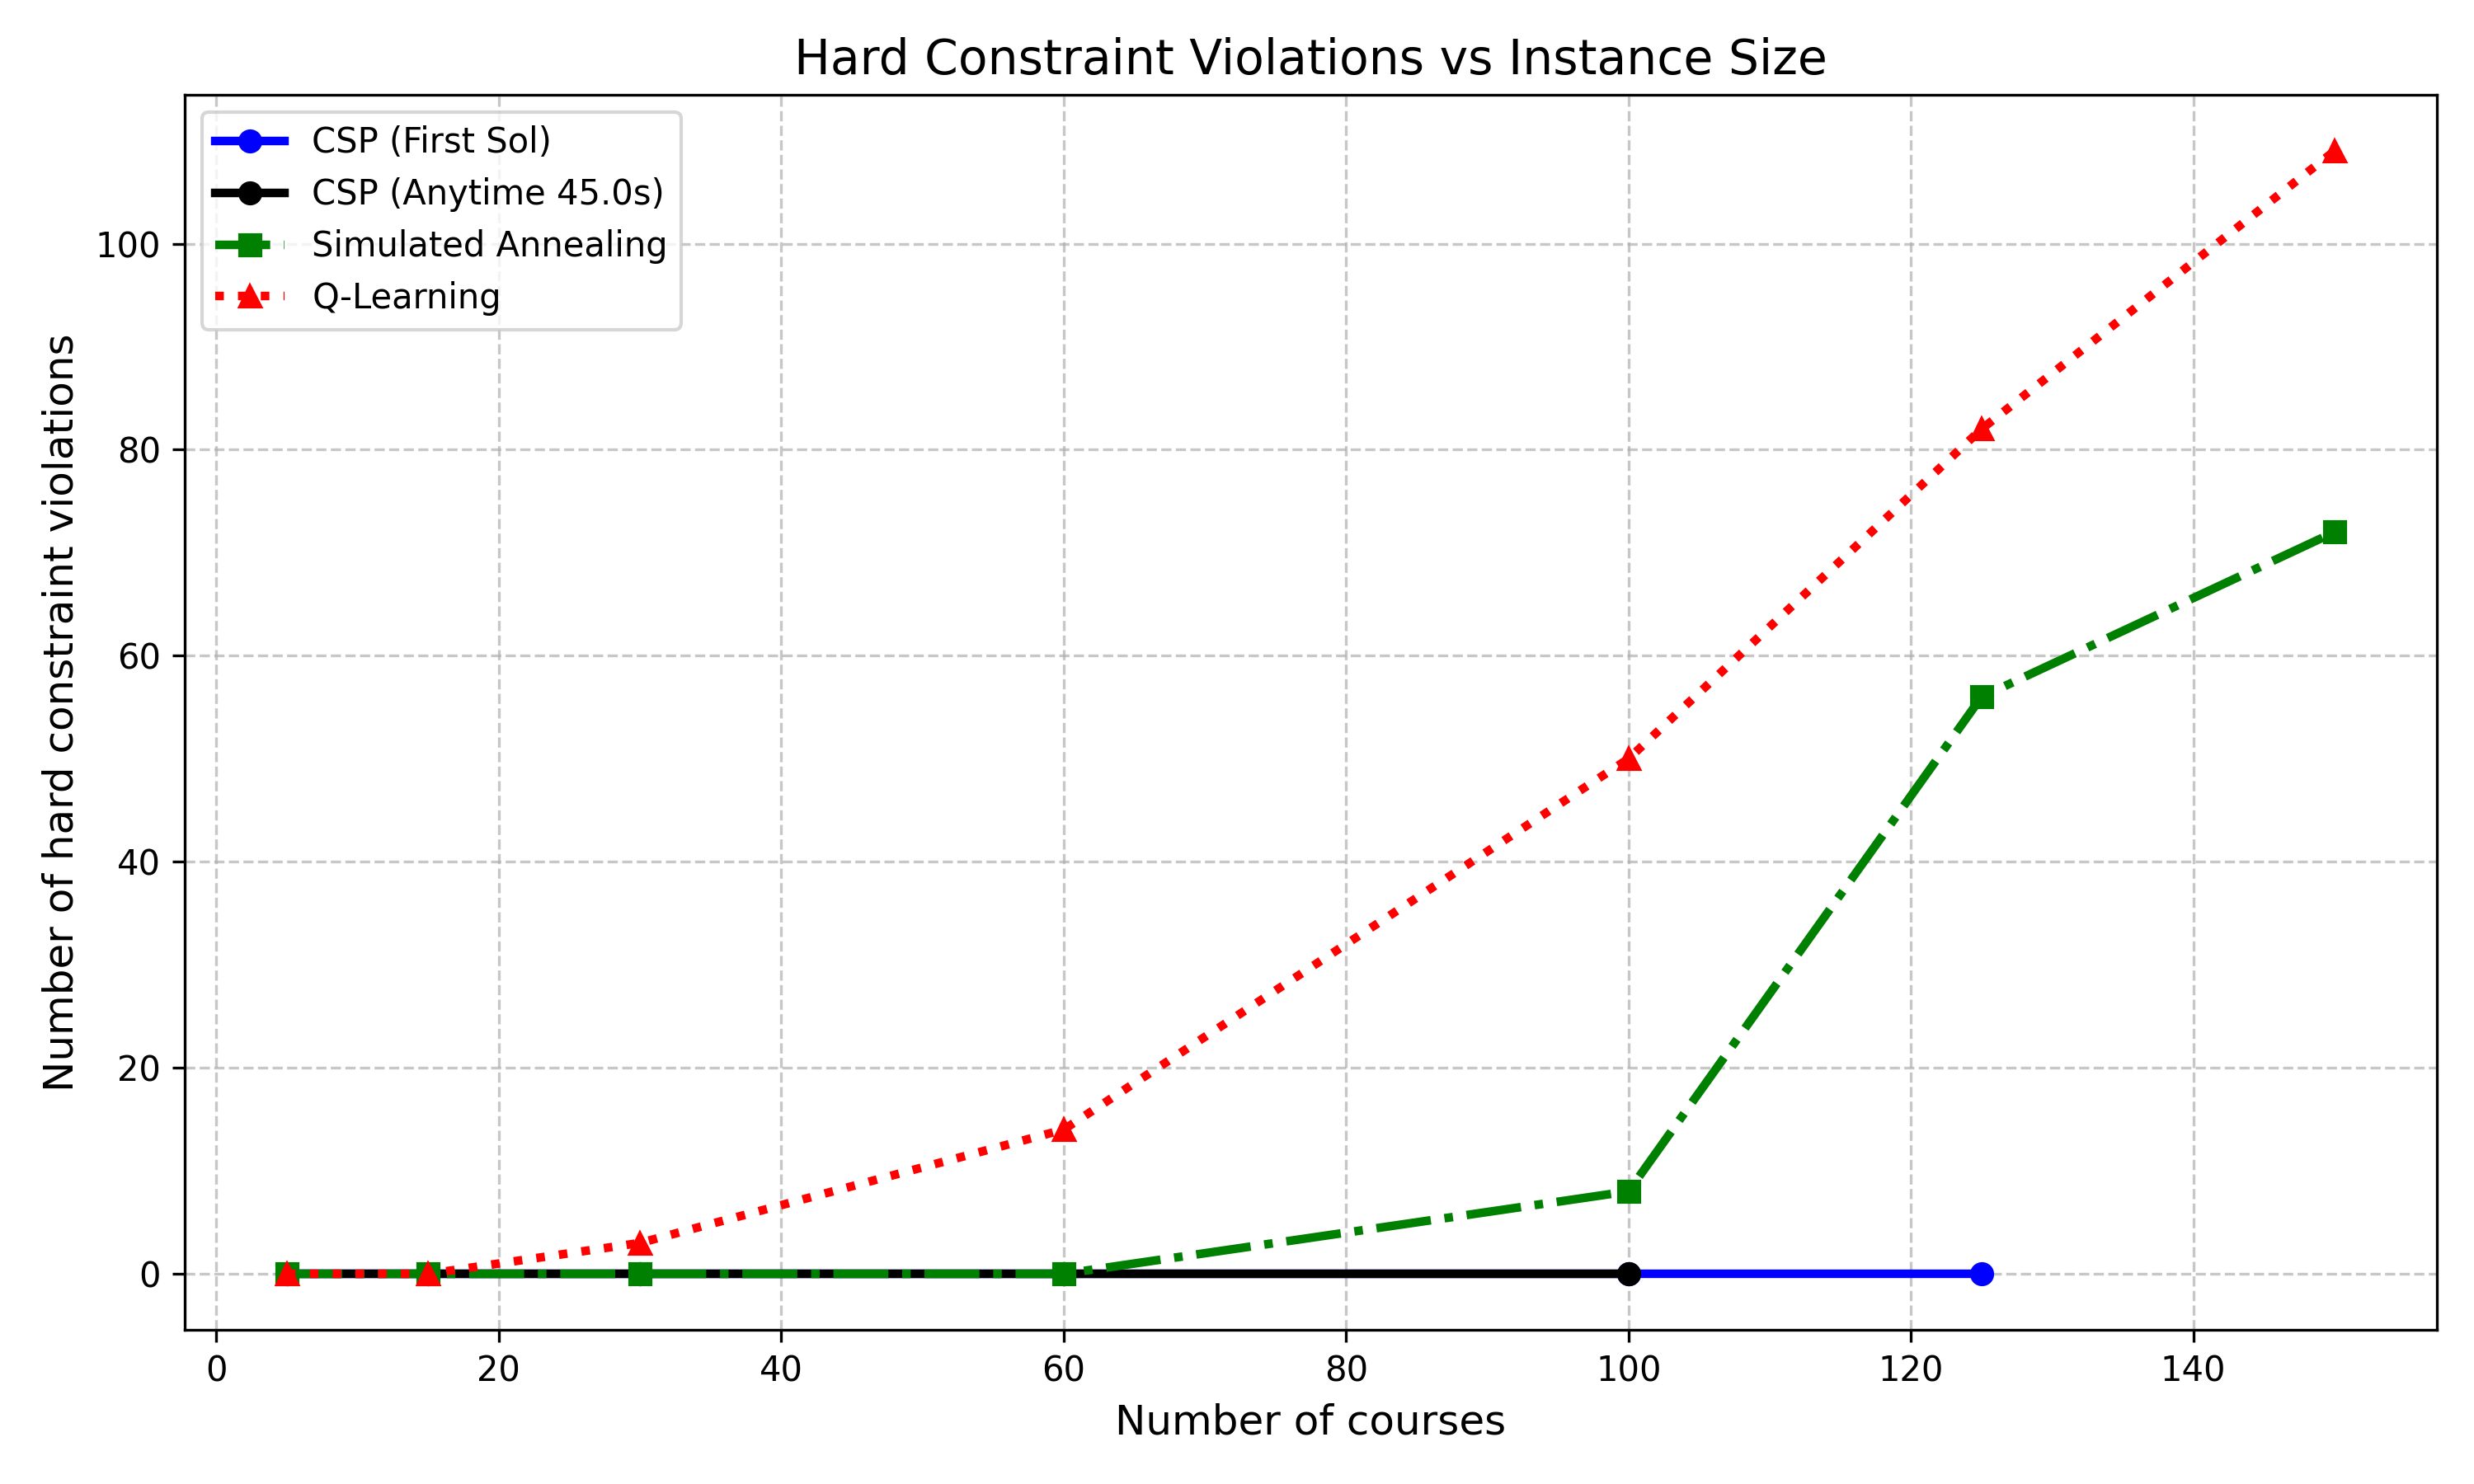
\includegraphics[width=0.95\columnwidth]{Images/violations.png}
\caption{Hard constraint violations vs.\ number of courses.}
\label{fig:viol}
\end{figure}

Figure~\ref{fig:viol} is the most diagnostic of the three plots. CSP never returns an invalid schedule by construction. SA accumulates violations progressively beyond 60 courses, reaching 72 at $n=150$. QL violations explode from $n=30$: without sufficient training, the agent places courses nearly at random, making it essentially unable to respect hard constraints at scale.

\section{Qualitative Comparison and Conclusion}

\subsection{Strengths and Weaknesses}

\begin{table}[h]
\centering
\caption{Qualitative comparison of the three approaches.}
\label{tab:comparison}
\small
\begin{tabular}{@{}lccc@{}}
\toprule
Criterion        & CSP            & SA             & Q-Learning \\
\midrule
Hard violations  & Always 0       & 0 up to 60c    & Grows from 30c \\
Soft score       & Highest        & Medium         & Low \\
Scalability      & Fails $>$125c  & Excellent      & Poor quality \\
Predictability   & Deterministic  & Stochastic     & Highly variable \\
Hard guarantee   & Yes            & No             & No \\
\bottomrule
\end{tabular}
\end{table}

The three approaches occupy clearly distinct positions in the trade-off space (Table~\ref{tab:comparison}). CSP is the right choice when constraint satisfaction is non-negotiable and the instance is of moderate size. It is also the most interpretable: the backtracking search is entirely deterministic, and observing zero backtracks provides direct evidence that the heuristics are working effectively. SA is the most practical all-round solver: it handles every instance size and always terminates, even if it cannot guarantee a violation-free result on very dense problems. Q-Learning, in its tabular form, is not suitable for production scheduling at the scale we tested. Its value in this project is academic: it illustrates why naive reinforcement learning struggles on combinatorial problems, and motivates the need for function approximation or hybrid approaches.

\subsection{Impact of Modelling Choices}

One observation worth highlighting is the role of modelling choices in explaining the results. The CSP's superior soft score (Figure~\ref{fig:soft}) is not an intrinsic algorithmic advantage: it is a direct consequence of sorting candidate assignments by soft score inside the LCV heuristic. Without this, the Anytime variant's iterative improvement would be far more valuable. Similarly, SA's lower soft score is a consequence of starting from a random initial schedule: the search must first eliminate hard violations (Figure~\ref{fig:viol}) before it can focus on optimising preferences, leaving fewer iterations for quality improvement. These modelling decisions matter as much as the choice of algorithm itself.

\subsection{Perspectives}

Two natural extensions emerge from this analysis. Using Q-Learning as a meta-heuristic selector for SA, choosing between Move and Swap operators at each step based on the current schedule state, would give QL a constant action space, bypassing the dimensionality problem entirely. Replacing the static MRV heuristic in CSP with a learned policy could also adaptively prioritise variables that are empirically harder to assign, potentially extending the scalability limit beyond 125 courses.

The empirical threshold between CSP viability and failure, located between 125 and 150 courses for our benchmark configuration (8 rooms, 20 slots), provides a concrete and reproducible data point for practitioners choosing between exact and heuristic scheduling methods.

\nocite{russell2020,claude}
\bibliography{references}

\end{document}
